\documentclass[12pt,titlepage]{article}
\usepackage[margin=1.25in]{geometry}
\usepackage{graphicx,amsmath,blindtext,minted,enumitem}

%% Variables definition
\newcommand{\vSubject}{Basic Programming Practicum}
\newcommand{\vSubtitle}{Jobsheet 9 Array 2}
\newcommand{\vName}{Dicha Zelianivan Arkana}
\newcommand{\vNIM}{2241720002}
\newcommand{\vClass}{1i}
\newcommand{\vDepartment}{Information Technology}
\newcommand{\vStudyProgram}{D4 Informatics Engineering}

%% [START] Tikz related stuff
\usepackage{tikz}
\usetikzlibrary{svg.path,calc,shapes.geometric,shapes.misc}
\tikzstyle{terminator} = [rectangle, draw, text centered, rounded corners = 1em, minimum height=2em]
\tikzstyle{preparation} = [chamfered rectangle, chamfered rectangle sep=0.75em, draw, text centered, minimum height = 2em]
\tikzstyle{process} = [rectangle, draw, text centered, minimum height=2em]
\tikzstyle{decision} = [diamond, aspect=2, draw, text centered, minimum height=2em]
\tikzstyle{data}=[trapezium, draw, text centered, trapezium left angle=60, trapezium right angle=120, minimum height=2em]
\tikzstyle{connector} = [line width=0.25mm,->]
%% [END] Tikz related stuff

%% [START] Fancy header related stuff
\usepackage{fancyhdr}
\pagestyle{fancy}
\setlength{\headheight}{15pt} % compensate fancyhdr style
\fancyhead{}
\fancyfoot{}
\fancyfoot[L]{\thepage}
\fancyfoot[R]{\textit{\vSubject - \vSubtitle}}
\renewcommand{\footrulewidth}{0.4pt}% default is 0pt, overline for footer
%% [END] Fancy header related stuff

%% [START] Custom tabular command related stuff
\usepackage{tabularx}
\newcommand{\details}[2]{
    #1 & #2  \\
}
%% [END] Custom tabular command related stuff

%% [START] Figure related stuff
\newcommand{\image}[3][1]{
    \begin{figure}[h]
        \centering
        \includegraphics[#1]{#2}
        \caption{#3}
        \label{#3}
    \end{figure}
}
%% [END] Figure related stuff

\begin{document}
\begin{titlepage}
    \centering
    \vfill
    {\bfseries\LARGE
        \vSubject\\
        \vskip0.25cm
        \vSubtitle
    }
    \vfill
    
\includegraphics[width=6cm]{images/polinema-logo.png}
    \vfill
    {
        \textbf{Name}\\
        \vName\\
        \vskip0.5cm
        \textbf{NIM}\\
        \vNIM\\
        \vskip0.5cm
        \textbf{Class}\\
        \vClass\\
        \vskip0.5cm
        \textbf{Department}\\
        \vDepartment\\
        \vskip0.5cm
        \textbf{Study Program}\\
        \vStudyProgram
    }
\end{titlepage}

\section{Laboratory}
\subsection{Experiment 1: Declare, Initialize, and Display 2D Array}
\begin{enumerate}
    \item Create a new project
    \item Create a new class, name it \textbf{Arr1}
    \item Write the basic structure of the Java programming language which contains the \texttt{main()} function
    \item {
        Create an array of integer type named \texttt{number} with a row capacity of 2 elements and a column of 3 elements

        \begin{minted}[autogobble]{java}
            int[][] number = new int[2][3];
        \end{minted}
    }
    \item {
        Fill in each element of the value array as follows:

        \begin{minted}[autogobble]{java}
            number[0][0] = 12;
            number[0][1] = 14;
            number[0][2] = 34;
            number[1][0] = 20;
            number[1][1] = 24;
            number[1][2] = 67;
        \end{minted}
    }
    \item {
        Display all contents of the elements to the screen

        \begin{minted}[autogobble]{java}
            System.out.println(number[0][0] + " " + number[0][1] + " " + number[0][2]);
            System.out.println(number[1][0] + " " + number[1][1] + " " + number[1][2]);
        \end{minted}
    }
    \pagebreak
    \item {
        Compile and run the program. Match the results of the running programs that you have created according to the following Display

        \begin{minted}[autogobble]{bash}
            12 14 34
            20 24 67
        \end{minted}

        \begin{figure}[h]
            \centering
            \fbox{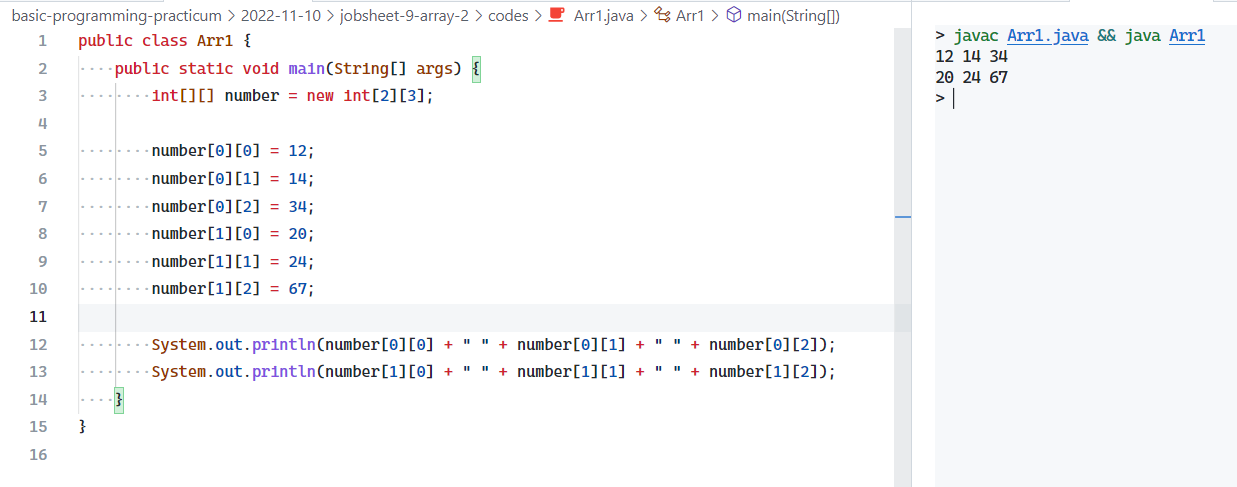
\includegraphics[width=.8\textwidth]{./images/arr1.png}}
            \caption{Experiment 1 code and output}
        \end{figure}
    }
\end{enumerate}

\subsubsection*{Questions!}
\begin{enumerate}
    \item {
        Should the array elements be filled sequentially? Explain!

        No. As long as the array has been initialised, we can fill it however we want. The order doesn't matter.
    }
    \item {
        In step 5, modify the code so that the filled elements are only array elements in odd row positions! Can this be done? Prove it!

        Yes, we can do this as shown on figure \ref{arr1-proof}

        \begin{figure}[h]
            \centering
            \fbox{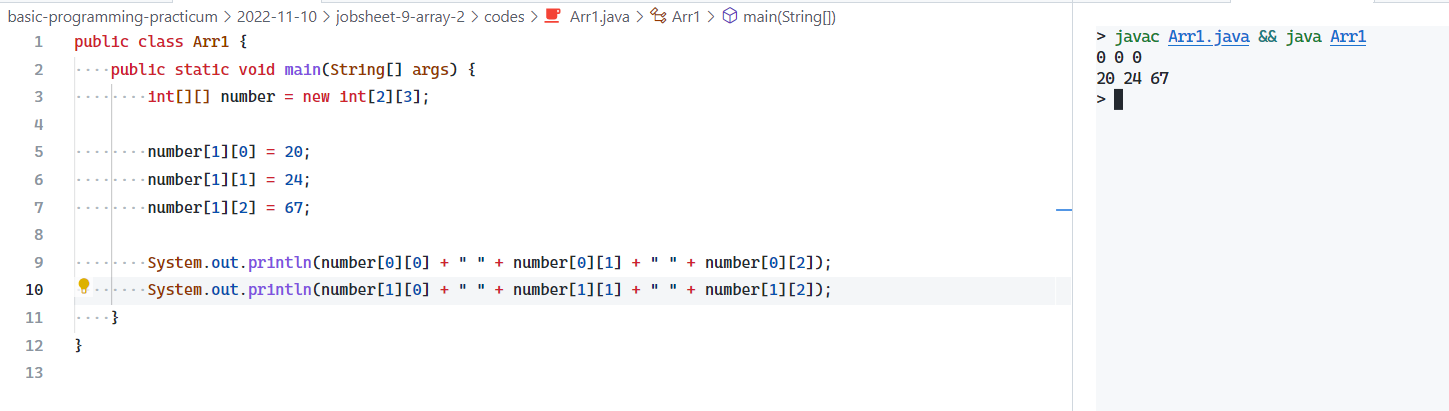
\includegraphics[width=.8\textwidth]{./images/arr1-proof.png}}
            \caption{Array with odd elements}
            \label{arr1-proof}
        \end{figure}
    }
\end{enumerate}

\subsection{Experiment 2: Display 2 Dimensional Array Elements Using Loop}
\begin{enumerate}
    \item Create a new class, name it \textbf{Arr2}
    \item Write the basic structure of the Java programming language which contains the \texttt{main()} function
    \item {
        Create an array of integer type named \texttt{number} with a row capacity of 2 elements and a column of 3 elements
        
        \begin{minted}[autogobble]{java}
            int[][] number = new int[2][3];
        \end{minted}
    }
    \item {
        Fill in each element of the value array as follows:

        \begin{minted}[autogobble]{java}
            number[0][0] = 12;
            number[0][1] = 14;
            number[0][2] = 34;
            number[1][0] = 20;
            number[1][1] = 24;
            number[1][2] = 67;
        \end{minted}
    }
    \item {
        Using a loop, display all the contents of the elements from the \texttt{number} array

        \begin{minted}[autogobble]{java}
            for (int i = 0; i < 2; i++) {
                for (int j = 0; j < 3; j++) {
                    System.out.print(number[i][j] + " ");
                }
                System.out.println("");
            }
        \end{minted}
    }
    \pagebreak
    \item {
        Compile and run the program. Match the results of the running programs that you have created according to the following Display

        \begin{minted}[autogobble]{bash}
            12 14 34
            20 24 67
        \end{minted}

        \begin{figure}[h]
            \centering
            \fbox{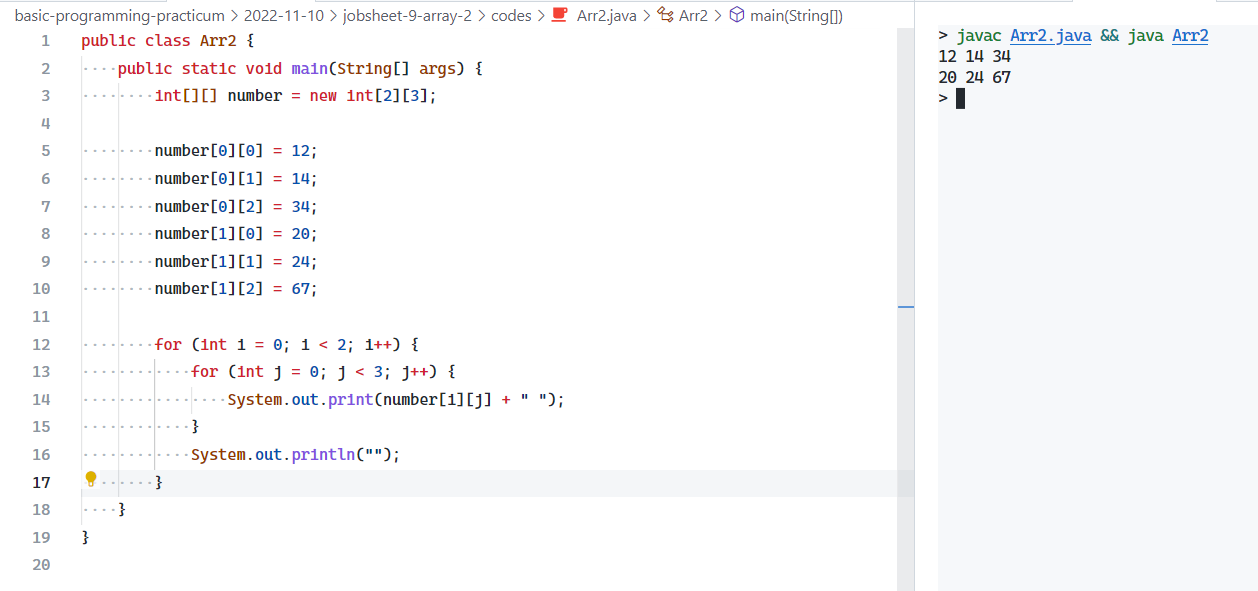
\includegraphics[width=.8\textwidth]{./images/arr2.png}}
            \caption{Experiment 2 code and output}
        \end{figure}
    }
\end{enumerate}

\pagebreak

\subsubsection*{Questions!}
\begin{enumerate}
    \item {
        How many columns was the array in Experiment 2? Change the number of columns to 4 so that the array declaration and instantiation looks like the following code
        
        \begin{minted}[autogobble]{java}
            int[][] number = new int[2][4];
        \end{minted}

        Then, fill in the array elements with any value, corresponding to the addition of these columns. Run the program again, what happened?

        \begin{itemize}
            \item There were 3 columns as shown by \texttt{int[2][3]}
            \item {
                The output still shows 2 rows and 3 columns (shown by figure \ref{arr2-col}) because we changed the number of rows but we didn't change the limit for the loop.

                \begin{figure}[h]
                    \centering
                    \fbox{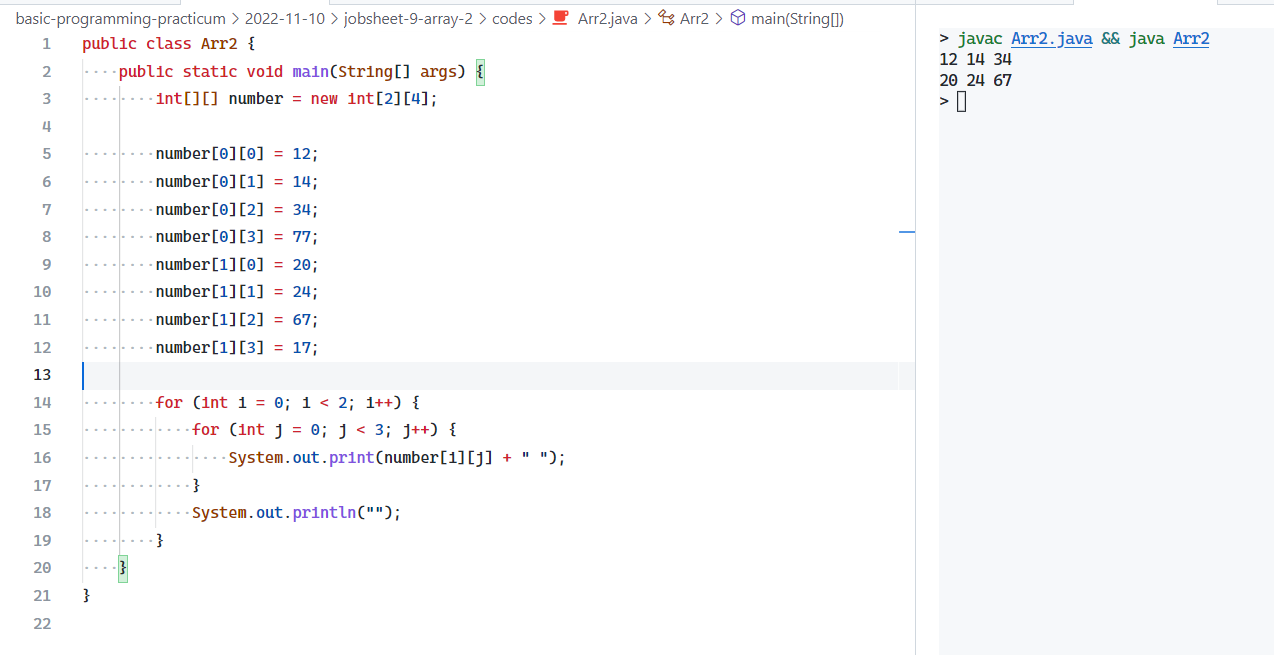
\includegraphics[width=.8\textwidth]{./images/arr2-col.png}}
                    \caption{Experiment 2 with 2 rows and 4 columns}
                    \label{arr2-col}
                \end{figure}
            }
        \end{itemize}
    }
    \item {
        In step 5, change the program code as follows

        \begin{minted}[autogobble]{java}
            for (int i = 0; i < number.length; i++) {
                for (int j = 0; j < number[0].length; j++) {
                    System.out.print(number[i][j] + " ");
                }
                System.out.println("");
            }
        \end{minted}

        Run the program after the change, what happened?

        The output will be the same. The reason is because we changed the hardcoded value to the length of the array.
        If we were to change the length of the array, we no longer need to update the loop because it will automatically gets the length of the array whether if it's 2, 3, 4, so on and so forth.
    }
    \item {
        Regarding displaying all array elements, change the program code to display array elements as follows

        \begin{minted}[autogobble]{java}
            for (int array[] : number) {
                for (int r : array) {
                    System.out.print(r + " ");
                }
                System.out.println("");
            }
        \end{minted}

        Run the results of these changes, what happened?

        The output is the same because we only changed the \texttt{for} loop into a \texttt{for-each} loop.
        In this case, they do the exact same thing. It's just an alternative way of doing what we did before using \texttt{for} loop.
    }
\end{enumerate}

\subsection{Experiment 3: Filling in 2 Dimensional Array Elements via Keyboard}
\begin{enumerate}
    \item Create a new class, name it \textbf{Arr3}
    \item Write the basic structure of the Java programming language which contains the \texttt{main()} function
    \item Add the Scanner library
    \item Make a \textbf{Scanner} declaration with the name \texttt{input}
    \item {
        Create an array of integer type named \texttt{number} with a row capacity of 2 elements and a column of 3 elements
        
        \begin{minted}[autogobble]{java}
            int[][] number = new int[2][3];
        \end{minted}
    }
    \item {
        Using a loop, create an input to fill in the \texttt{number} array element

        \begin{minted}[autogobble]{java}
            for (int i = 0; i < number.length; i++) {
                for (int j = 0; j < number[0].length; j++) {
                    System.out.print("Enter a number [" + i + "][" + j + "]: ");
                    number[i][j] = input.nextInt();
                }
                System.out.println("---------------");
            }
        \end{minted}
    }
    \item {
        Using a loop, display all the contents of the elements from the \texttt{number} array

        \begin{minted}[autogobble]{java}
            for (int i = 0; i < number.length; i++) {
                for (int j = 0; j < number[0].length; j++) {
                    System.out.print(number[i][j] + " ");
                }
                System.out.println("");
            }
        \end{minted}
    }
    \item {
        Compile and run the program. Match the results of the running programs that you have created according to the following Display

        \begin{minted}[autogobble]{bash}
            Enter a number [0][0]: 7
            Enter a number [0][1]: 3
            Enter a number [0][2]: 9
            ---------------
            Enter a number [1][0]: 11
            Enter a number [1][1]: 4
            Enter a number [1][2]: 2
            ---------------
            7 3 9
            11 4 2
        \end{minted}

        \begin{figure}[h]
            \centering
            \fbox{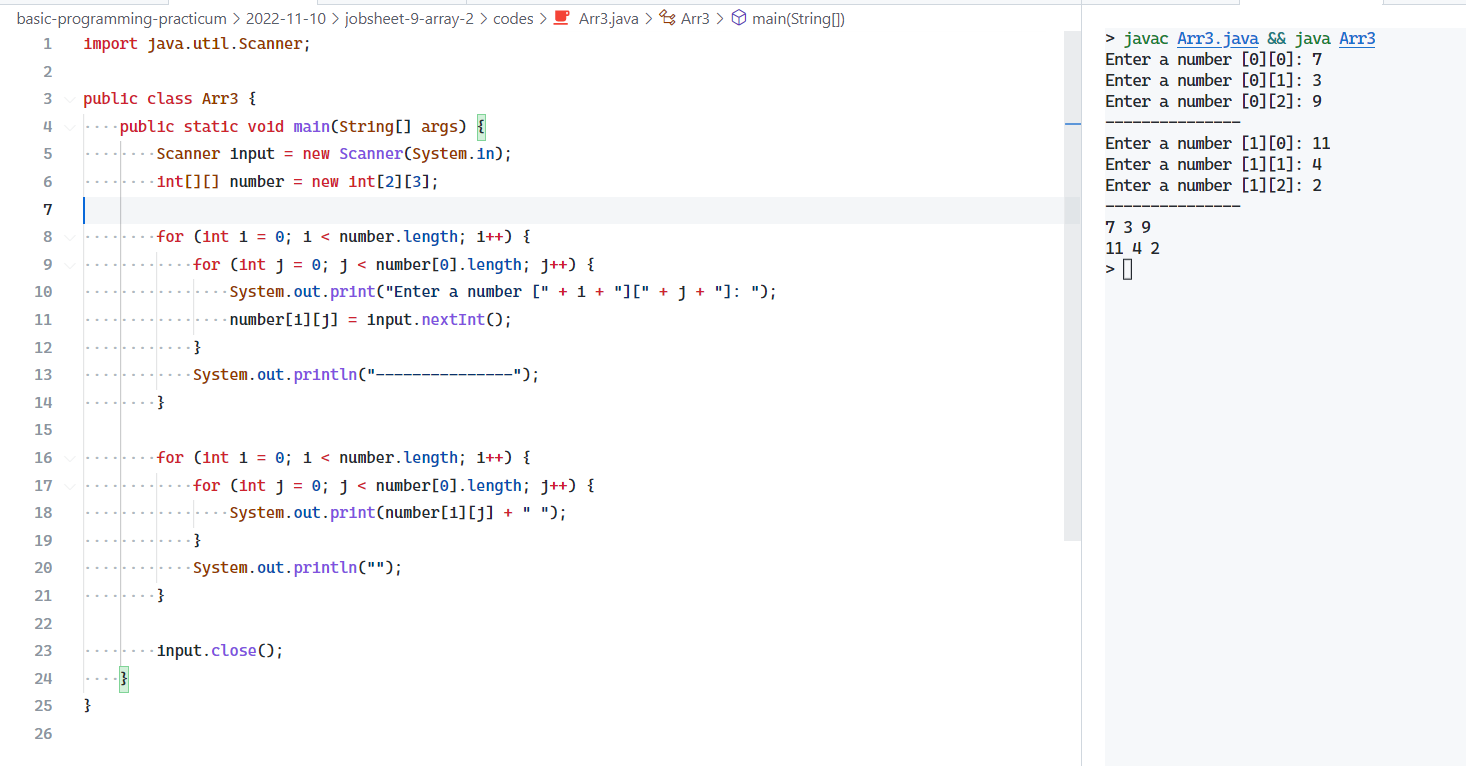
\includegraphics[width=.8\textwidth]{./images/arr3.png}}
            \caption{Experiment 3 code and output}
        \end{figure}
    }
\end{enumerate}

\pagebreak

\subsubsection*{Questions!}
\begin{enumerate}
    \item {
        In step 6 can position j be replaced with position i? Explain!

        Yes, it can, but the result will be flipped. The row becomes the column and vice versa.
    }
    \item {
        Add program code to determine the number of rows and columns of array elements dynamically (rows and columsn are determined when the program runs through the keyboard)!

        \begin{figure}[h]
            \centering
            \fbox{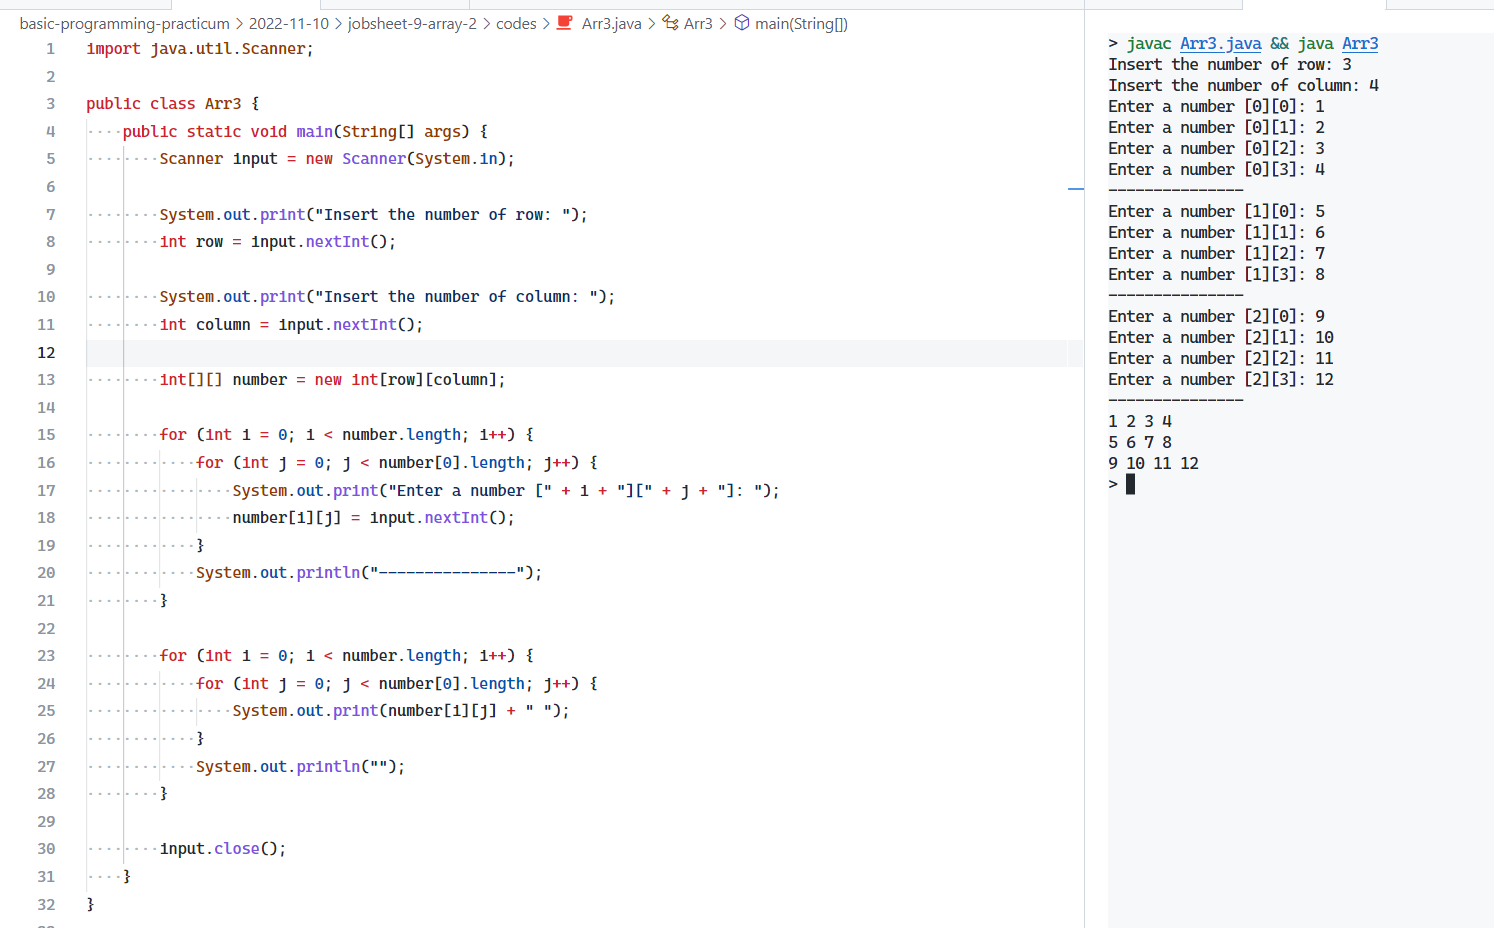
\includegraphics[width=.65\textwidth]{./images/arr3-dynamic.png}}
            \caption{Experiment 3 with dynamic rows and columns from the user input}
        \end{figure}
    }
    \item {
        Modify the program code to display array elements using \texttt{foreach}!

        \begin{figure}[h]
            \centering
            \fbox{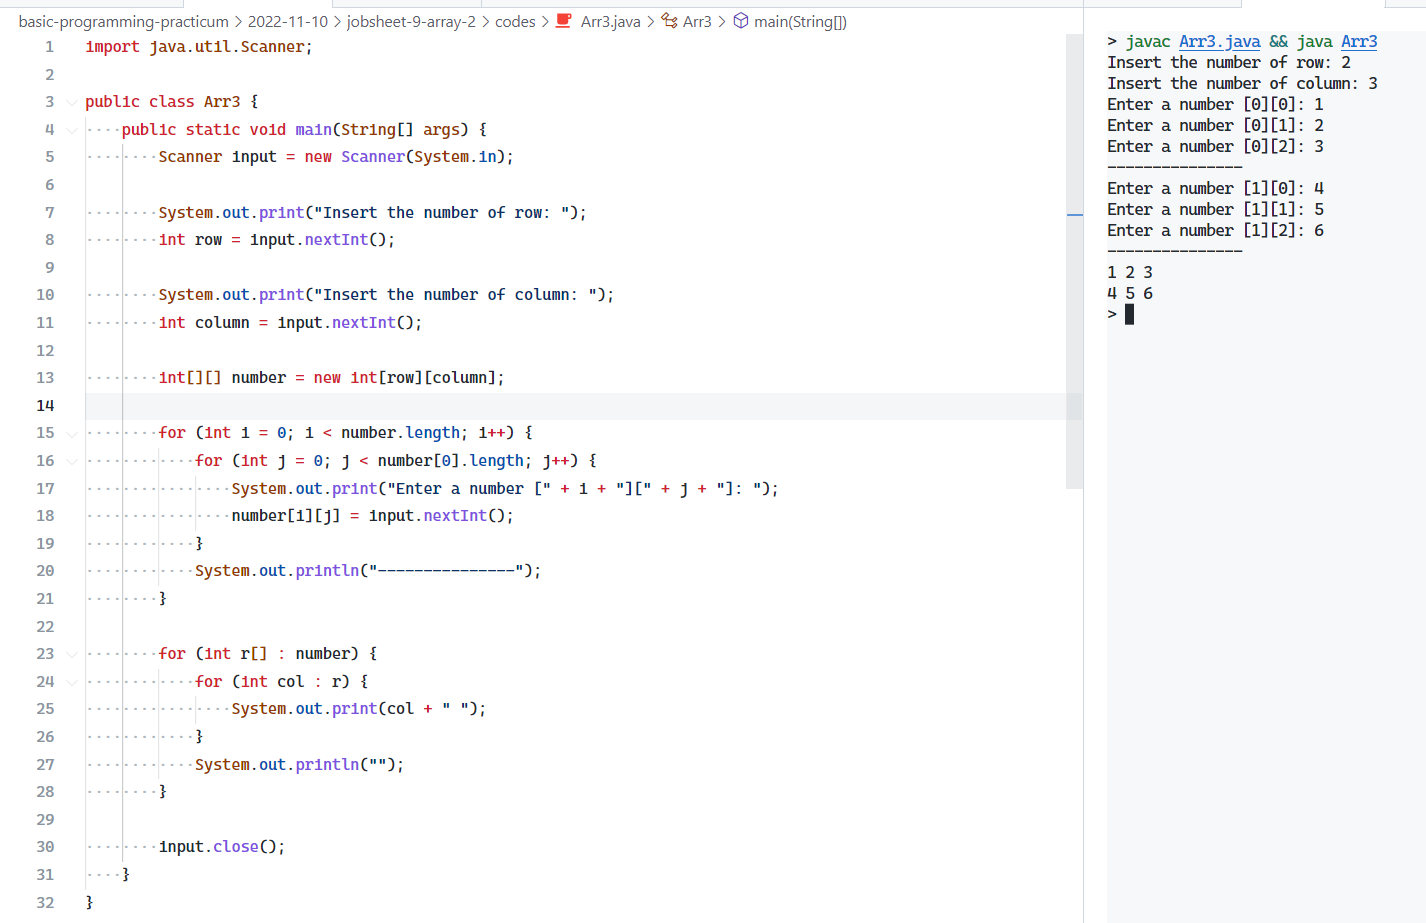
\includegraphics[width=.65\textwidth]{./images/arr3-foreach.png}}
            \caption{Experiment 3 using foreach instead of for-loop}
        \end{figure}
    }
\end{enumerate}

\pagebreak

\section{Assignment}
\begin{enumerate}
    \item {
        Create a program that has two arrays as follows:
        \begin{itemize}
            \item The first array is a one-dimensional array \texttt{char code[10]}, containing the license plate codes
            \item The second array is a two-dimensional array containing the city names which are paired with the license plate codes
        \end{itemize}
        The illustration of the array display is as follows
        \begin{table*}[h]
            \centering
            \ttfamily \begin{tabular}[h]{|c|c|c|c|c|c|c|c|c|c|c|c|}
                \cline{1-1} \cline{3-12}
                A & ~ & B & A & N & T & E & N & ~ & ~ & ~ & ~ \\
                \cline{1-1} \cline{3-12}
                B & ~ & J & A & K & A & R & T & A & ~ & ~ & ~ \\
                \cline{1-1} \cline{3-12}
                D & ~ & B & A & N & D & U & N & G & ~ & ~ & ~ \\
                \cline{1-1} \cline{3-12}
                E & ~ & C & I & R & E & B & O & N & ~ & ~ & ~ \\
                \cline{1-1} \cline{3-12}
                F & ~ & B & O & G & O & R & ~ & ~ & ~ & ~ & ~ \\
                \cline{1-1} \cline{3-12}
                G & ~ & P & E & K & A & L & O & N & G & A & N \\
                \cline{1-1} \cline{3-12}
                H & ~ & S & E & M & A & R & A & N & G & ~ & ~ \\
                \cline{1-1} \cline{3-12}
                L & ~ & S & U & R & A & B & A & Y & A & ~ & ~ \\
                \cline{1-1} \cline{3-12}
                N & ~ & M & A & L & A & N & G & ~ & ~ & ~ & ~ \\
                \cline{1-1} \cline{3-12}
                T & ~ & T & E & G & A & L & ~ & ~ & ~ & ~ & ~ \\
                \cline{1-1} \cline{3-12}
            \end{tabular}
        \end{table*}

        \begin{figure}[h]
            \centering
            \fbox{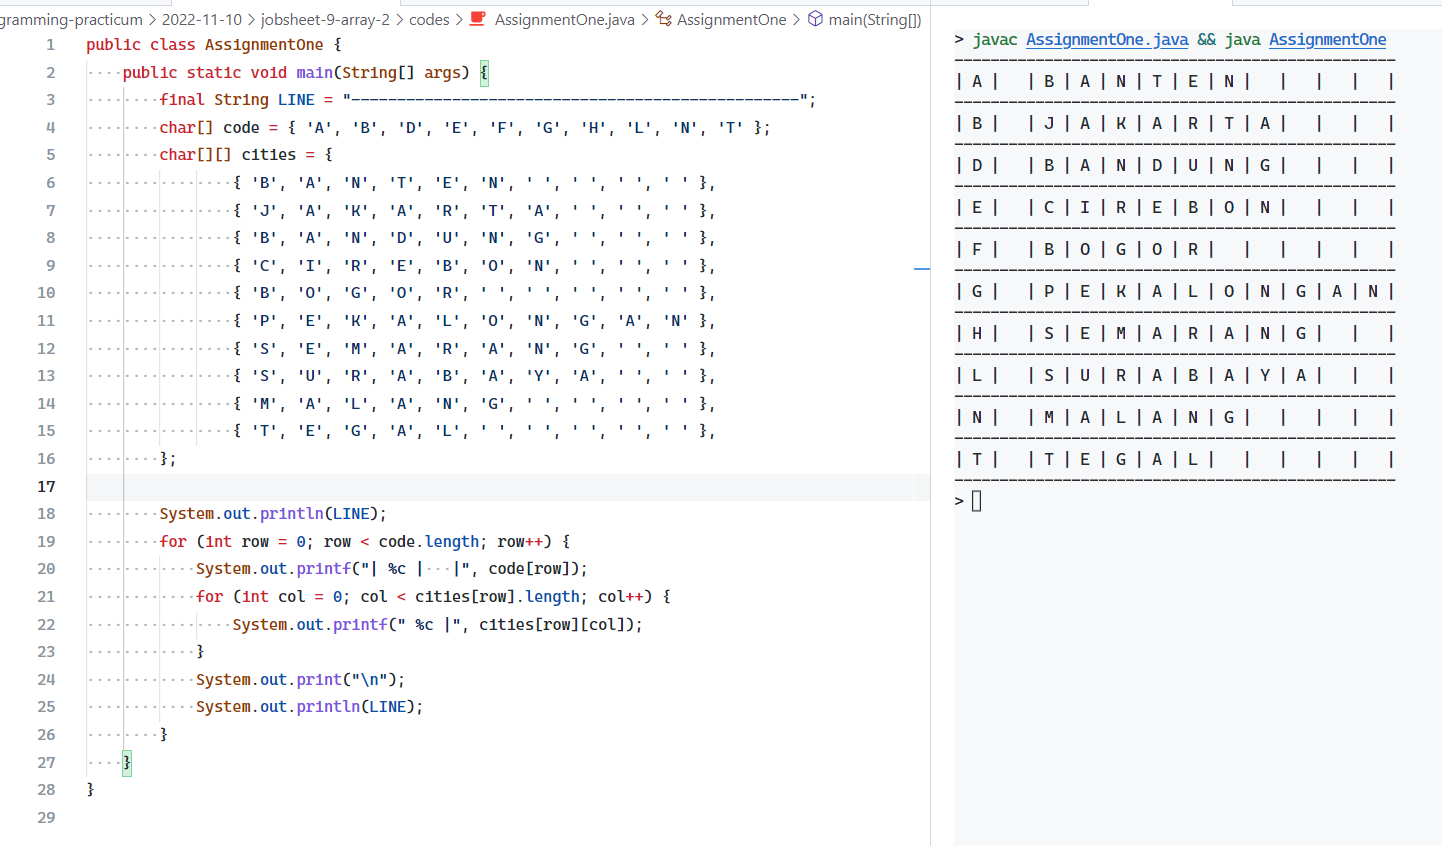
\includegraphics[width=.65\textwidth]{./images/assignment-one.png}}
            \caption{Assignment 1 code and output}
        \end{figure}
    }
    \pagebreak
    \item {
        Create a program containing a two-dimensional array having the row and column sizes obtained from keyboard input.
        Then, make input to fill the array elements. Next, make a menu choice that consists of:
        \begin{enumerate}[label=\alph*.]
            \item \textbf{MIN Value}. Display the value of the smallest array element to the screen
            \item \textbf{MIN Value \& Amount}. Display to the screen the smallest value and how many the smallest value is, and also display the row and column location of the minimum value.
            \item \textbf{Array conditions}. Display the word "FOUND" on the screen if there is a value of 50 between the two-dimensional array elements, otherwise print the word "NOT FOUND".
        \end{enumerate}

        \large{\textbf{Code}}
        \begin{minted}[autogobble,fontsize=\footnotesize]{java}
            import java.util.Scanner;

            public class AssignmentTwo {
                public static void main(String[] args) {
                    Scanner input = new Scanner(System.in);

                    System.out.print("Insert the number of row: ");
                    int row = input.nextInt();
                    System.out.print("Insert the number of column: ");
                    int col = input.nextInt();
                    int[][] numbers = new int[row][col];

                    // store the variable ahead of time so we don't need to calculate it on demand
                    int minValue = Integer.MAX_VALUE;
                    int minValueAmount = 0;
                    String minValuePosition = "";
                    final int MAX_NUM = 50;
                    boolean isBigNumberFound = false;

                    for (int r = 0; r < numbers.length; r++) {
                        for (int c = 0; c < numbers[r].length; c++) {
                            System.out.printf("Insert the number for row %d and column %d: ", r, c);
                            int inputValue = input.nextInt();
                            numbers[r][c] = inputValue;

                            if (inputValue <= minValue) {
                                // reset since the max number changed
                                if (inputValue != minValue) {
                                    minValueAmount = 0;
                                    minValuePosition = "";
                                }

                                minValue = inputValue;
                                if (inputValue == minValue) {
                                    minValuePosition += String.format(
                                        "%d -> [row: %d, col: %d]\n",
                                        minValueAmount + 1, r, c
                                    );
                                    minValueAmount++;
                                }
                            }

                            if (inputValue > MAX_NUM) {
                                isBigNumberFound = true;
                            }
                        }
                    }

                    int chosenMenu;
                    while (true) {
                        System.out.println("Menu:");
                        System.out.println("1. Display MIN Value");
                        System.out.println("2. Display MIN Value & Amount");
                        System.out.println("3. Array conditions");
                        System.out.print("Choose which menu to open (1-3): ");
                        chosenMenu = input.nextInt();
                        if (chosenMenu >= 1 && chosenMenu <= 3) break;
                        System.out.println("Please insert the menu number correctly!");
                    }

                    switch (chosenMenu) {
                        case 1:
                            System.out.printf("The MIN value is: %d\n", minValue);
                            break;
                        case 2:
                            System.out.printf("The MIN value is: %d\n", minValue);
                            System.out.printf("The MIN value amount is: %d\n", minValueAmount);
                            System.out.printf("The MIN value position is: \n%s\n", minValuePosition);
                            break;
                        case 3:
                            System.out.println(isBigNumberFound ? "FOUND" : "NOT FOUND");
                            break;
                    }

                    input.close();
                }
            }

        \end{minted}

        \pagebreak

        \large{\textbf{Output}}
        \begin{figure}[h]
            \centering
            \fbox{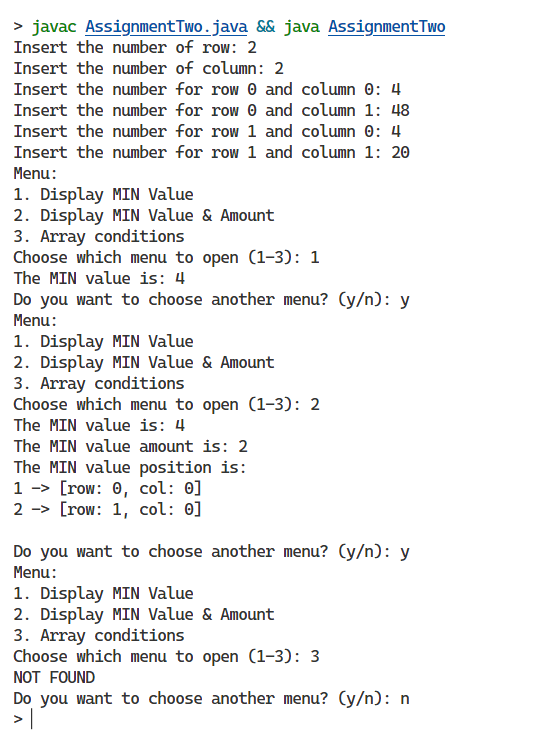
\includegraphics[width=.7\textwidth]{./images/assignment-two-output.png}}
            \caption{Assignment 2 output}
        \end{figure}
    }
\end{enumerate}

\end{document}

